\documentclass[tikz,border=5pt]{standalone}
\usepackage{tikz}
\usepackage{amsmath,amssymb}
\usetikzlibrary{arrows.meta,positioning,shapes.geometric,fit,backgrounds,calc,decorations.pathreplacing}

% Colors (colorblind-safe)
\definecolor{busblue}{HTML}{4682B4}
\definecolor{genorange}{HTML}{E69F00}
\definecolor{loadgreen}{HTML}{009E73}
\definecolor{xfmrpurple}{HTML}{CC79A7}
\definecolor{ipoptdark}{HTML}{2C3E50}
\definecolor{procblue}{HTML}{D4E6F1}
\definecolor{boxgray}{HTML}{E8E8E8}
\definecolor{nores}{HTML}{D55E00}
\definecolor{improvblue}{HTML}{0072B2}

\begin{document}
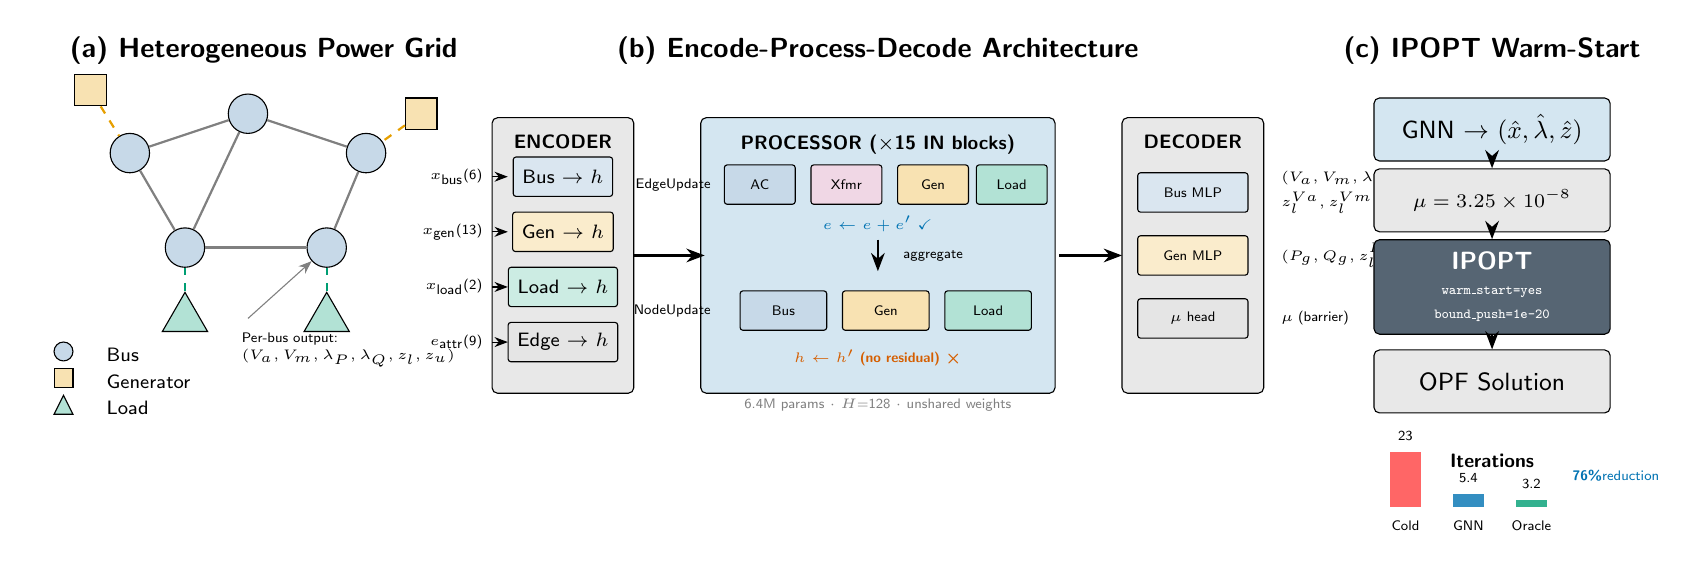
\begin{tikzpicture}[
    >=Stealth,
    node distance=0.4cm,
    every node/.style={font=\sffamily\small},
    block/.style={rectangle, draw, rounded corners=2pt, minimum height=0.8cm, align=center},
    smallblock/.style={rectangle, draw, rounded corners=1pt, minimum height=0.5cm, minimum width=1.2cm, align=center, font=\sffamily\scriptsize},
]

% ============================================================
% PANEL (a): Problem Setup
% ============================================================
\begin{scope}[local bounding box=panelA]

% Title
\node[font=\sffamily\bfseries] at (2.2, 5.8) {(a) Heterogeneous Power Grid};

% Grid graph
\node[circle, draw, fill=busblue!30, minimum size=0.5cm] (b1) at (0.5, 4.5) {};
\node[circle, draw, fill=busblue!30, minimum size=0.5cm] (b2) at (2.0, 5.0) {};
\node[circle, draw, fill=busblue!30, minimum size=0.5cm] (b3) at (3.5, 4.5) {};
\node[circle, draw, fill=busblue!30, minimum size=0.5cm] (b4) at (1.2, 3.3) {};
\node[circle, draw, fill=busblue!30, minimum size=0.5cm] (b5) at (3.0, 3.3) {};

\node[rectangle, draw, fill=genorange!30, minimum size=0.4cm] (g1) at (0.0, 5.3) {};
\node[rectangle, draw, fill=genorange!30, minimum size=0.4cm] (g2) at (4.2, 5.0) {};

\node[regular polygon, regular polygon sides=3, draw, fill=loadgreen!30, minimum size=0.35cm] (l1) at (1.2, 2.4) {};
\node[regular polygon, regular polygon sides=3, draw, fill=loadgreen!30, minimum size=0.35cm] (l2) at (3.0, 2.4) {};

% AC lines
\draw[thick, gray] (b1) -- (b2);
\draw[thick, gray] (b2) -- (b3);
\draw[thick, gray] (b1) -- (b4);
\draw[thick, gray] (b4) -- (b5);
\draw[thick, gray] (b3) -- (b5);
\draw[thick, gray] (b2) -- (b4);

% Gen links
\draw[dashed, genorange, thick] (g1) -- (b1);
\draw[dashed, genorange, thick] (g2) -- (b3);

% Load links
\draw[dashed, loadgreen, thick] (l1) -- (b4);
\draw[dashed, loadgreen, thick] (l2) -- (b5);

% Legend
\node[font=\sffamily\scriptsize] at (0.4, 1.6) {
\begin{tabular}{cl}
\tikz\draw[fill=busblue!30] (0,0) circle (0.12); & Bus \\
\tikz\draw[fill=genorange!30] (0,0) rectangle (0.24,0.24); & Generator \\
\tikz\draw[fill=loadgreen!30] (0,0) -- (0.12,0.24) -- (0.24,0) -- cycle; & Load \\
\end{tabular}
};

% Output annotation
\node[font=\sffamily\tiny, align=left, anchor=west] at (1.8, 2.0) {
Per-bus output:\\
$(V_a, V_m, \lambda_P, \lambda_Q, z_l, z_u)$
};
\draw[->, thin, gray] (2.0, 2.4) -- (b5);

\end{scope}

% ============================================================
% PANEL (b): EPD Architecture
% ============================================================
\begin{scope}[xshift=5.5cm, local bounding box=panelB]

% Title
\node[font=\sffamily\bfseries] at (4.5, 5.8) {(b) Encode-Process-Decode Architecture};

% Encoder box
\node[block, fill=boxgray, minimum width=1.8cm, minimum height=3.5cm] (enc) at (0.5, 3.2) {};
\node[font=\sffamily\scriptsize\bfseries, anchor=north] at (0.5, 4.85) {ENCODER};
\node[smallblock, fill=busblue!20] at (0.5, 4.2) {Bus $\to$ $h$};
\node[smallblock, fill=genorange!20] at (0.5, 3.5) {Gen $\to$ $h$};
\node[smallblock, fill=loadgreen!20] at (0.5, 2.8) {Load $\to$ $h$};
\node[smallblock, fill=gray!20] at (0.5, 2.1) {Edge $\to$ $h$};

% Input labels
\node[font=\sffamily\tiny, anchor=east] at (-0.4, 4.2) {$x_{\text{bus}}$(6)};
\node[font=\sffamily\tiny, anchor=east] at (-0.4, 3.5) {$x_{\text{gen}}$(13)};
\node[font=\sffamily\tiny, anchor=east] at (-0.4, 2.8) {$x_{\text{load}}$(2)};
\node[font=\sffamily\tiny, anchor=east] at (-0.4, 2.1) {$e_{\text{attr}}$(9)};
\draw[->, thin] (-0.4, 4.2) -- (-0.2, 4.2);
\draw[->, thin] (-0.4, 3.5) -- (-0.2, 3.5);
\draw[->, thin] (-0.4, 2.8) -- (-0.2, 2.8);
\draw[->, thin] (-0.4, 2.1) -- (-0.2, 2.1);

% Processor box
\node[block, fill=procblue, minimum width=4.5cm, minimum height=3.5cm] (proc) at (4.5, 3.2) {};
\node[font=\sffamily\scriptsize\bfseries, anchor=north] at (4.5, 4.85) {PROCESSOR ($\times$15 IN blocks)};

% Inside processor: one IN block expanded
% Edge update row
\node[smallblock, fill=busblue!30, minimum width=0.9cm] (eu1) at (3.0, 4.1) {\tiny AC};
\node[smallblock, fill=xfmrpurple!30, minimum width=0.9cm] (eu2) at (4.1, 4.1) {\tiny Xfmr};
\node[smallblock, fill=genorange!30, minimum width=0.9cm] (eu3) at (5.2, 4.1) {\tiny Gen};
\node[smallblock, fill=loadgreen!30, minimum width=0.9cm] (eu4) at (6.2, 4.1) {\tiny Load};
\node[font=\sffamily\tiny, anchor=east] at (2.5, 4.1) {Edge\\Update};

% Residual on edges
\node[font=\sffamily\tiny, text=improvblue] at (4.5, 3.6) {$e \leftarrow e + e'$ \textcolor{improvblue}{\checkmark}};

% Arrow down
\draw[->, thick] (4.5, 3.4) -- (4.5, 3.0);
\node[font=\sffamily\tiny, anchor=west] at (4.7, 3.2) {aggregate};

% Node update row
\node[smallblock, fill=busblue!30, minimum width=1.1cm] (nu1) at (3.3, 2.5) {\tiny Bus};
\node[smallblock, fill=genorange!30, minimum width=1.1cm] (nu2) at (4.6, 2.5) {\tiny Gen};
\node[smallblock, fill=loadgreen!30, minimum width=1.1cm] (nu3) at (5.9, 2.5) {\tiny Load};
\node[font=\sffamily\tiny, anchor=east] at (2.5, 2.5) {Node\\Update};

% NO residual on nodes (key finding!)
\node[font=\sffamily\tiny, text=nores, font=\sffamily\tiny\bfseries] at (4.5, 1.9) {$h \leftarrow h'$ (no residual) \textcolor{nores}{$\boldsymbol{\times}$}};

% Decoder box
\node[block, fill=boxgray, minimum width=1.8cm, minimum height=3.5cm] (dec) at (8.5, 3.2) {};
\node[font=\sffamily\scriptsize\bfseries, anchor=north] at (8.5, 4.85) {DECODER};
\node[smallblock, fill=busblue!20, minimum width=1.4cm] at (8.5, 4.0) {\tiny Bus MLP};
\node[smallblock, fill=genorange!20, minimum width=1.4cm] at (8.5, 3.2) {\tiny Gen MLP};
\node[smallblock, fill=gray!20, minimum width=1.4cm] at (8.5, 2.4) {\tiny $\mu$ head};

% Output labels
\node[font=\sffamily\tiny, anchor=west, align=left] at (9.5, 4.0) {$(V_a, V_m, \lambda_P, \lambda_Q,$\\$z_{l}^{Va}, z_{l}^{Vm}, z_{u}^{Va}, z_{u}^{Vm})$};
\node[font=\sffamily\tiny, anchor=west] at (9.5, 3.2) {$(P_g, Q_g, z_l^{Pg}, z_l^{Qg}, z_u^{Pg}, z_u^{Qg})$};
\node[font=\sffamily\tiny, anchor=west] at (9.5, 2.4) {$\mu$ (barrier)};

% Arrows between sections
\draw[->, thick] (1.4, 3.2) -- (2.3, 3.2);
\draw[->, thick] (6.8, 3.2) -- (7.6, 3.2);

% Dimension annotation
\node[font=\sffamily\tiny, gray] at (4.5, 1.3) {6.4M params $\cdot$ $H$=128 $\cdot$ unshared weights};

\end{scope}

% ============================================================
% PANEL (c): IPOPT Warm-Start Pipeline
% ============================================================
\begin{scope}[xshift=16cm, local bounding box=panelC]

% Title
\node[font=\sffamily\bfseries] at (1.8, 5.8) {(c) IPOPT Warm-Start};

% GNN prediction box
\node[block, fill=procblue, minimum width=3cm] (gnn) at (1.8, 4.8) {GNN $\to$ $(\hat{x}, \hat{\lambda}, \hat{z})$};

% mu
\node[block, fill=boxgray, minimum width=3cm, font=\sffamily\scriptsize] (mu) at (1.8, 3.9) {$\mu = 3.25 \times 10^{-8}$};

% IPOPT box
\node[block, fill=ipoptdark!80, text=white, minimum width=3cm, minimum height=1.2cm, align=center] (ipopt) at (1.8, 2.8) {\textbf{IPOPT}\\[-2pt]\tiny\texttt{warm\_start=yes}\\[-2pt]\tiny\texttt{bound\_push=1e-20}};

% Solution
\node[block, fill=boxgray, minimum width=3cm] (sol) at (1.8, 1.6) {OPF Solution};

% Arrows
\draw[->, thick] (gnn) -- (mu);
\draw[->, thick] (mu) -- (ipopt);
\draw[->, thick] (ipopt) -- (sol);

% Comparison bars (simplified)
\node[font=\sffamily\scriptsize\bfseries, anchor=north] at (1.8, 0.8) {Iterations};
\fill[red!60] (0.5, 0.0) rectangle (0.9, 0.7);
\fill[improvblue!80] (1.3, 0.0) rectangle (1.7, 0.17);
\fill[loadgreen!80] (2.1, 0.0) rectangle (2.5, 0.10);
\node[font=\sffamily\tiny, anchor=north] at (0.7, -0.05) {Cold};
\node[font=\sffamily\tiny, anchor=north] at (1.5, -0.05) {GNN};
\node[font=\sffamily\tiny, anchor=north] at (2.3, -0.05) {Oracle};
\node[font=\sffamily\tiny, anchor=south] at (0.7, 0.72) {23};
\node[font=\sffamily\tiny, anchor=south] at (1.5, 0.19) {5.4};
\node[font=\sffamily\tiny, anchor=south] at (2.3, 0.12) {3.2};

% Reduction annotation
\node[font=\sffamily\tiny, text=improvblue, anchor=west] at (2.7, 0.4) {\textbf{76\%}\\reduction};

\end{scope}

\end{tikzpicture}
\end{document}
